\documentclass[11pt]{article}
\usepackage{latexsym}
\usepackage{amsmath}
\usepackage{amssymb}
\usepackage{amsthm}
\usepackage{epsfig}
\usepackage{psfig}

\newcommand{\handout}[5]{
  \noindent
  \begin{center}
  \framebox{
    \vbox{
      \hbox to 5.78in { {\bf 6.851: Advanced Data Structures } \hfill #2 }
      \vspace{4mm}
      \hbox to 5.78in { {\Large \hfill #5  \hfill} }
      \vspace{2mm}
      \hbox to 5.78in { {\em #3 \hfill #4} }
    }
  }
  \end{center}
  \vspace*{4mm}
}

\newcommand{\lecture}[4]{\handout{#1}{#2}{#3}{Scribe: #4}{Lecture #1}}

\newtheorem{theorem}{Theorem}
\newtheorem{corollary}[theorem]{Corollary}
\newtheorem{lemma}[theorem]{Lemma}
\newtheorem{observation}[theorem]{Observation}
\newtheorem{proposition}[theorem]{Proposition}
\newtheorem{definition}[theorem]{Definition}
\newtheorem{claim}[theorem]{Claim}
\newtheorem{fact}[theorem]{Fact}
\newtheorem{assumption}[theorem]{Assumption}

% 1-inch margins, from fullpage.sty by H.Partl, Version 2, Dec. 15, 1988.
\topmargin 0pt
\advance \topmargin by -\headheight
\advance \topmargin by -\headsep
\textheight 8.9in
\oddsidemargin 0pt
\evensidemargin \oddsidemargin
\marginparwidth 0.5in
\textwidth 6.5in

\parindent 0in
\parskip 1.5ex
%\renewcommand{\baselinestretch}{1.25}

\begin{document}

\lecture{2 --- 02/09, 2012}{Spring 2012}{Prof.\ Erik Demaine}{Erek Speed, Victor Jakubiuk}

\section{Overview}

The main idea of persistent data structures is that when a change is made in the past, an entirely new universe is obtained. A more science-fiction approach to time travel is that you can make a change in the past and see its results not only in the current state of the data structure, but also all the changes in between the past and now.

We maintain one timeline of updates and queries for a persistent data structure:

\begin{figure*}[h]
  \centering
  \leavevmode
  \scalebox{.5}{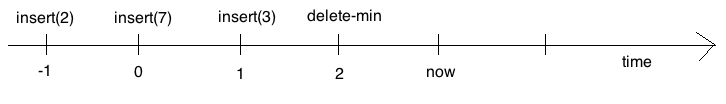
\includegraphics{timeline.png}}
\end{figure*}



Usually, operations are appended at the end of the timeline (present time). With retroactive data structures we can do that in the past too.

\section{Retroactivity}

The following operations are supported by retroactive DS:

\begin{itemize}
\item {\em Insert(t, update)} - inserts operation ``update'' at time $t$
\item {\em Delete(t)} - deletes the operation at time $t$
\item {\em Query(t, query)} - queries the DS with a ``query'' at time $t$
\end{itemize}

Uppercase Insert indicates an operation on retroactive DS, lowercase update is the operation on the actual DS.

You can think of time $t$ as integers, but a better approach is to use an order-maintanance DS to avoid using non-integers (in case you want to insert an operation between times $t$ and $t+1$), as mentioned in the first lecture.

There are three types of retroactivity:
\begin{itemize}
\item {\em Partial} - Query always done at $t = \infty$ (now)
\item {\em Full} - Query at any time $t$ (possibly in the past)
\item {\em Nonoblivious} - Insert, Delete, Query at any time $t$, also if an operation modifies DS, we must say which future queries are changed.
\end{itemize}

\subsection{Easy case with commutativity and inversions}

Assume the following hold:
\begin{itemize}
\item {\em Commutative updates:} $x.y = y.x$ ($x$ followed by $y$ is the same as $y$ followed by $x$); that is the updates can be reordered $\Rightarrow$ Insert(t, op) = Insert(now, op).
\item {\em Invertible updates:} There exists an operation $x^{-1}$, such that $x.x^{-1} = \emptyset \Rightarrow$ Delete(t, op) = Insert(now, op$^{-1}$)
\end{itemize}

\subsubsection{Partial retroactivity}

These two assumptions allow us to solve some retroactive problems easily, such as:
\begin{itemize}
\item {\em hashing} 
\item {\em array} with operation $A[i] += \Delta$ (but no direct assignment)
\end{itemize}

\subsection{Full retroactivity}

First, lets define the {\bf search problem}: maintain set $S$ of objects, subject to insert, delete, query($x, S$).

{\bf Decomposable search problem} [1980, 2007]: same as the search problem, with a restriction that the query must satisfy:
query($x, A \cup B) = f($query$(x, A), $query($x, B))$, for some function $f$ computed in $O(1)$ (sets $A$ and $B$ may overlap). Examples of problems with such a function include:

\begin{itemize}
\item {\em Dynamic nearest neighbor}
\item {\em Successor on a line}
\item {\em Point location}
\end{itemize}

{\bf Claim}: Full Retroactivity for decomposable search problems (with commutativity and inversions) can be done in $O(\lg{m})$ factor overhead both in time and space (where $m$ is the number of operations) using {\bf segment tree} [1980, Bentley and Saxon (??)]

\begin{figure*}[h]
  \centering
  \leavevmode
  \scalebox{.5}{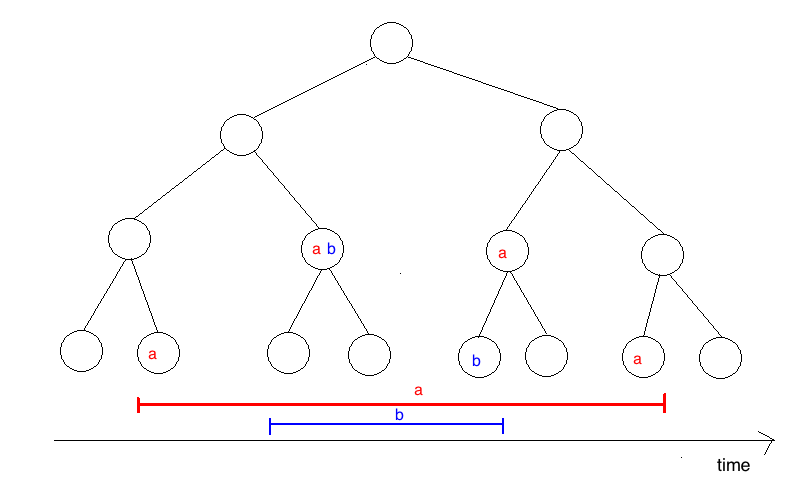
\includegraphics{segment_tree.png}}
  \caption{Segment Tree}
\end{figure*}

We want to build a balanced search tree on time (leaves represent time). Every element ``lives'' in the data structure on the interval of time, corresponding to its insertion and deletion. Each element appears in $\lg{n}$ nodes.

To query on this tree at time $t$, we want to know what operations have been done on this tree from the beginning of time to $t$. Because the query is decomposable, we can look at $\lg{n}$ different nodes and combine the results (using the function $f$). 

\subsection{General case of full retroactivity}

{\bf Roll back method}: 
\begin{itemize}
\item write down a (linear) chain of operations and queries
\item change $r$ time units in the past with factor $O(r)$ overhead. 
\end{itemize}

That's the best we can do in general. 

Lower bound: $\Omega (r)$ overhead necessary.

Proof: Data Structure maintains 2 values (registers): $X$ and $Y$, initially $\emptyset$. The following operations are supported: $X = x$, $Y += \Delta$, $Y = X.Y$, query '$Y?$'. Perform the following operations (Cramer's rule):
$$Y += a_n, X = X.Y, Y += a_{n-1}, X = X.Y, \ldots, Y += a_0$$


which is equivalent to computing $$Y = a_n X^{n} + a_{n-1} X^{n-1} + ... + a_0$$

Now, execute Insert($t = 0, X=x$), which changes where the polynomial is evaluated. This cannot be done faster than re-evaluating the polynomial. In history-independent algebraict decision tree, for any field, independent of pre-processing of the coefficients, need $\Omega(n)$ field operations (result from 2001), where $n$ is the degree of the polynomial.

\subsection{Cell-probe problem}

How many integers (words) of memory do you need to read to solve your problem? (gives a lower bound on running time).

Claim: $\Omega(\sqrt{\frac{r}{\lg{r}}})$.

Open problem: $\Omega(r)$.

Proof of the lower bound claim:
\begin{itemize}
\item DS maintans $n$ words (integers of $w \ge \lg{n}$ bits). 
\item Arithmetic operations are allowed. 
\item Query = what is the value of an integer?
\item Compute FFT. 
\item Retroactively change the words $\Rightarrow$ Dynamic FFT. 
\item Changing $x_i$ requires $\Omega(\sqrt{n})$ cell probes.
\end{itemize}

\subsection{Intermediate setting}

Priority queues...




\subsection{Blah blah blah}
Here is a subsection.

\subsubsection{Blah blah blah}
Here is a subsubsection. You can use these as well.

\subsection{Using Boldface}
Make sure to use lots of boldface.

\paragraph{Question:}
How would you use boldface?

\paragraph{Example:}
This is an example showing how to use boldface to 
help organize your lectures.


\paragraph{Some Formatting.}
Here is some formatting that you can use in your notes:
\begin{itemize}
\item {\em Item One} -- This is the first item.
\item {\em Item Two} -- This is the second item.
\item \dots and here are other items.
\end{itemize}

If you need to number things, you can use this style:
\begin{enumerate}
\item {\em Item One} -- Again, this is the first item.
\item {\em Item Two} -- Again, this is the second item.
\item \dots and here are other items.
\end{enumerate}

\paragraph{Bibliography.}
Please give real bibliographical citations for the papers that we
mention in class. See below for how to include a bibliography section.
If you use BibTeX, integrate the .bbl file into your .tex
source. You should reference papers like this: ``The FKS
dictionary originates in a paper by Fredman, Koml\'{o}s and
Szemer\'{e}di \cite{fks}.'' In general, the name of the authors should
appear in text at most once (for the first citation); further
citations look like: ``Our proof follows that of \cite{fks}''.

Take a look at previous lectures (TeX files are available) to see the
details. A excellent source for bibliographical citations is
DBLP. Just Google DBLP and an author's name.


%\bibliography{mybib}
\bibliographystyle{alpha}

\begin{thebibliography}{77}

\bibitem{fks}
M. Fredman, J. Koml\'{o}s, E. Szemer\'{e}di,
\emph{Storing a Sparse Table with $O(1)$ Worst Case Access Time},
Journal of the ACM, 31(3):538-544, 1984.

\end{thebibliography}

\end{document}
